\documentclass[a4paper,dvipsnames]{article}

\input ../header
\newcommand{\checkedbox}{\makebox[0pt][l]{$\square$}\raisebox{.15ex}{\hspace{0.1em}$\checkmark$}}
\newcommand{\checkbox}{\makebox[0pt][l]{$\square$}\raisebox{.15ex}{\hspace{0.1em}}\hspace{3mm}}

\begin{document}

\title{Évaluation 7 -- Sujet A}
\author{}
\date{}

\maketitle{}

\pagestyle{empty}
\thispagestyle{empty}

% Exercices sur les identités remarquables (factoriser)
\exo[3 points] Factoriser les expressions suivantes. Préciser à chaque fois l'identité remarquable utilisée.
\begin{enumerate}
  \item Identité remarquable utilisée : \dotfill\\
    \[x^2-10x+25=\hdots\hdots\hdots\hdots\hdots\hdots\]
  \item Identité remarquable utilisée : \dotfill\\
    \[4x^2-36=\hdots\hdots\hdots\hdots\hdots\hdots\]
\end{enumerate}

\bigskip

% Exercices sur les quotients
\exo[3 points] Réduire au même dénominateur afin d'écrire les expressions suivantes sous la forme d'un unique quotient.
\begin{multicols}{2}
  \begin{enumerate}
    \item $5x+\dfrac{2x^2}{2x+1}$
    \item $\dfrac{-2x}{2x+1}+\dfrac{3x+2}{x+1}$
  \end{enumerate}
\end{multicols}
\dotfill\rep{22}

\bigskip

% Exercice sur la boucle for
\exo[2 points] \vspace{-2mm}
\begin{enumerate}
  \item Préciser les valeurs prises par \mintinline{python}{k} dans la boucle \mintinline{python}{for k in range(6):}.\rep{3}
  \item Quelle boucle peut-on écrire pour qu'une variable \mintinline{python}{i} prenne les valeurs $2$, $3$, $4$, $5$, $6$ ?\rep{3}
\end{enumerate}

\pagebreak

% Exercice de géométrie avec les identités remarquables
\exo[4 points] Dans la figure suivante, $ABCD$ et $EFGH$ sont des rectangles. La \og{}bande\fg{} $ABCGFEHD$ est de largeur constante notée $x$. De plus $AB=10$ et $BC=7$. On note $\mathcal{A}(x)$ l'aire du rectangle $EFGH$.

\begin{center}
  \psset{xunit=1.0cm,yunit=1.0cm,algebraic=true,dimen=middle,dotstyle=o,dotsize=5pt 0,linewidth=1.pt,arrowsize=3pt 2,arrowinset=0.25}
  \begin{pspicture*}(0.,0.)(10.,7.)
    \psline[linewidth=1.pt](1.,1.)(1.,6.)
    \psline[linewidth=1.pt](1.,6.)(9.,6.)
    \psline[linewidth=1.pt](9.,6.)(9.,1.)
    \psline[linewidth=1.pt](1.,1.)(9.,1.)
    \psline[linewidth=1.pt](2.,6.)(2.,2.)
    \psline[linewidth=1.pt](2.,2.)(8.,2.)
    \psline[linewidth=1.pt](8.,2.)(8.,6.)
    \uput[d](1,1){$A$}
    \uput[d](9,1){$B$}
    \uput[ur](9,6){$C$}
    \uput[ul](1,6){$D$}
    \uput[d](2,2){$E$}
    \uput[d](8,2){$F$}
    \uput[ul](8,6){$G$}
    \uput[ur](2,6){$H$}
    \psline{<->}(1,6.2)(2,6.2)
    \uput[u](1.5,6.2){$x$}
    \psline{<->}(8,6.2)(9,6.2)
    \uput[u](8.5,6.2){$x$}
    \psline{<->}(0.8,1)(0.8,2)
    \uput[l](0.8,1.5){$x$}
  \end{pspicture*}
\end{center}

\begin{enumerate}
  \item Justifier que $\mathcal{A}(x)=(10-2x)(7-x)$.\rep{6}
  \item Développer et réduire $\mathcal{A}(x)$.\rep{6}
    % A(x) = 2x^2 -24x + 70
  \item Prouver que $\mathcal{A}(x)=2(x-6)^2-2$.\rep{8}
\end{enumerate}

\bigskip

% Exercice sur les vecteurs
\exo[2 points] Tracer deux vecteurs ayant :
\begin{multicols}{2}
  \begin{enumerate}
    \item la même direction, la même longueur et pas le même sens
      \begin{center}
	\psset{xunit=0.7cm,yunit=0.7cm,algebraic=true,dimen=middle,dotstyle=o,dotsize=5pt 0,linewidth=2.pt,arrowsize=3pt 2,arrowinset=0.25}
	\begin{pspicture*}(1.,1.)(7.,7.)
	  \multips(0,1)(0,1.0){7}{\psline[linestyle=dashed,linecap=1,dash=1.5pt 1.5pt,linewidth=0.4pt,linecolor=lightgray]{c-c}(1.,0)(7.,0)}
	  \multips(1,0)(1.0,0){7}{\psline[linestyle=dashed,linecap=1,dash=1.5pt 1.5pt,linewidth=0.4pt,linecolor=lightgray]{c-c}(0,1.)(0,7.)}
	  \psaxes[labelFontSize=\scriptstyle,xAxis=true,yAxis=true,Dx=1.,Dy=1.,ticksize=-2pt 0,subticks=2]{->}(0,0)(1.,1.)(7.,7.)
      \end{pspicture*}
      \end{center}
    \item la même direction, le même sens et pas la même longueur
      \begin{center}
	\psset{xunit=0.7cm,yunit=0.7cm,algebraic=true,dimen=middle,dotstyle=o,dotsize=5pt 0,linewidth=2.pt,arrowsize=3pt 2,arrowinset=0.25}
	\begin{pspicture*}(1.,1.)(7.,7.)
	  \multips(0,1)(0,1.0){7}{\psline[linestyle=dashed,linecap=1,dash=1.5pt 1.5pt,linewidth=0.4pt,linecolor=lightgray]{c-c}(1.,0)(7.,0)}
	  \multips(1,0)(1.0,0){7}{\psline[linestyle=dashed,linecap=1,dash=1.5pt 1.5pt,linewidth=0.4pt,linecolor=lightgray]{c-c}(0,1.)(0,7.)}
	  \psaxes[labelFontSize=\scriptstyle,xAxis=true,yAxis=true,Dx=1.,Dy=1.,ticksize=-2pt 0,subticks=2]{->}(0,0)(1.,1.)(7.,7.)
      \end{pspicture*}
      \end{center}
%    \item la même direction mais pas la même longueur, ni le même sens
%      \begin{center}
%	\psset{xunit=0.7cm,yunit=0.7cm,algebraic=true,dimen=middle,dotstyle=o,dotsize=5pt 0,linewidth=2.pt,arrowsize=3pt 2,arrowinset=0.25}
%	\begin{pspicture*}(1.,1.)(7.,7.)
%	  \multips(0,1)(0,1.0){7}{\psline[linestyle=dashed,linecap=1,dash=1.5pt 1.5pt,linewidth=0.4pt,linecolor=lightgray]{c-c}(1.,0)(7.,0)}
%	  \multips(1,0)(1.0,0){7}{\psline[linestyle=dashed,linecap=1,dash=1.5pt 1.5pt,linewidth=0.4pt,linecolor=lightgray]{c-c}(0,1.)(0,7.)}
%	  \psaxes[labelFontSize=\scriptstyle,xAxis=true,yAxis=true,Dx=1.,Dy=1.,ticksize=-2pt 0,subticks=2]{->}(0,0)(1.,1.)(7.,7.)
%      \end{pspicture*}
%      \end{center}
%    \item la même longueur, mais pas la même direction
%      \begin{center}
%	\psset{xunit=0.7cm,yunit=0.7cm,algebraic=true,dimen=middle,dotstyle=o,dotsize=5pt 0,linewidth=2.pt,arrowsize=3pt 2,arrowinset=0.25}
%	\begin{pspicture*}(1.,1.)(7.,7.)
%	  \multips(0,1)(0,1.0){7}{\psline[linestyle=dashed,linecap=1,dash=1.5pt 1.5pt,linewidth=0.4pt,linecolor=lightgray]{c-c}(1.,0)(7.,0)}
%	  \multips(1,0)(1.0,0){7}{\psline[linestyle=dashed,linecap=1,dash=1.5pt 1.5pt,linewidth=0.4pt,linecolor=lightgray]{c-c}(0,1.)(0,7.)}
%	  \psaxes[labelFontSize=\scriptstyle,xAxis=true,yAxis=true,Dx=1.,Dy=1.,ticksize=-2pt 0,subticks=2]{->}(0,0)(1.,1.)(7.,7.)
%      \end{pspicture*}
%      \end{center}
  \end{enumerate}
\end{multicols}

\bigskip

\exo[2 points] Soient $A$, $B$ et $C$ trois points. En utilisant la relation de Chasles, compléter chacune des égalités suivantes :
\begin{multicols}{4}
  \begin{enumerate}
    \item $\vect{BA}+\vect{\hdots C}=\vect{BC}$
    \item $\vect{AB}+\vect{\vphantom{A}B\hdots}=\vect{AC}$
    \item $\vect{C\hdots}+\vect{BA}=\vect{CA}$
    \item $\vect{\hdots C}+\vect{\hdots A}=\vect{BA}$
  \end{enumerate}
\end{multicols}

\bigskip

\exo[2 points] Sur chacune des figures suivantes, construire le vecteur $\vect{u}+\vect{v}$. On fera apparaître sur la construction les vecteurs $\vect{u}$ et $\vect{v}$ représentés \og{}bout à bout\fg{}.

\medskip

\begin{multicols}{2}
  \begin{enumerate}
    \item[]
      \NormalCoor
      \psset{xunit=0.7cm,yunit=0.7cm,algebraic=true,dimen=middle,dotstyle=o,dotsize=5pt 0,linewidth=1.pt,arrowsize=3pt 2,arrowinset=0.25}
      \begin{pspicture*}(0.,0.)(10.,10.)
	\multips(0,0)(0,1.0){11}{\psline[linestyle=dashed,linecap=1,dash=1.5pt 1.5pt,linewidth=0.4pt,linecolor=lightgray]{c-c}(0.,0)(10.,0)}
	\multips(0,0)(1.0,0){11}{\psline[linestyle=dashed,linecap=1,dash=1.5pt 1.5pt,linewidth=0.4pt,linecolor=lightgray]{c-c}(0,0.)(0,10.)}
	\psline[linecolor=blue]{->}(1,1)(4,2)
	\psline[linecolor=red]{->}(3,5)(6,2)
	\uput[d](2.5,1.5){$\color{blue}\vect{v}$}
	\uput[u](4.5,3.5){$\color{red}\vect{u}$}
      \end{pspicture*}
    \item[]
      \NormalCoor
      \psset{xunit=0.7cm,yunit=0.7cm,algebraic=true,dimen=middle,dotstyle=o,dotsize=5pt 0,linewidth=1.pt,arrowsize=3pt 2,arrowinset=0.25}
      \begin{pspicture*}(0.,0.)(10.,10.)
	\multips(0,0)(0,1.0){11}{\psline[linestyle=dashed,linecap=1,dash=1.5pt 1.5pt,linewidth=0.4pt,linecolor=lightgray]{c-c}(0.,0)(10.,0)}
	\multips(0,0)(1.0,0){11}{\psline[linestyle=dashed,linecap=1,dash=1.5pt 1.5pt,linewidth=0.4pt,linecolor=lightgray]{c-c}(0,0.)(0,10.)}
	\psline[linecolor=blue]{->}(1,1)(2,6)
	\psline[linecolor=red]{->}(4,4)(7,4)
	\uput[l](1.5,3.5){$\color{blue}\vect{v}$}
	\uput[u](5.5,4){$\color{red}\vect{u}$}
      \end{pspicture*}
%    \item[]
%      \NormalCoor
%      \psset{xunit=0.7cm,yunit=0.7cm,algebraic=true,dimen=middle,dotstyle=o,dotsize=5pt 0,linewidth=1.pt,arrowsize=3pt 2,arrowinset=0.25}
%      \begin{pspicture*}(0.,0.)(10.,10.)
%	\multips(0,0)(0,1.0){11}{\psline[linestyle=dashed,linecap=1,dash=1.5pt 1.5pt,linewidth=0.4pt,linecolor=lightgray]{c-c}(0.,0)(10.,0)}
%	\multips(0,0)(1.0,0){11}{\psline[linestyle=dashed,linecap=1,dash=1.5pt 1.5pt,linewidth=0.4pt,linecolor=lightgray]{c-c}(0,0.)(0,10.)}
%	\psline[linecolor=blue]{->}(3,8)(4,2)
%	\psline[linecolor=red]{->}(7,4)(1,2)
%	\uput[l](3,8){$\color{blue}\vect{v}$}
%	\uput[u](7,4){$\color{red}\vect{u}$}
%      \end{pspicture*}
%    \item[]
%      \NormalCoor
%      \psset{xunit=0.7cm,yunit=0.7cm,algebraic=true,dimen=middle,dotstyle=o,dotsize=5pt 0,linewidth=1.pt,arrowsize=3pt 2,arrowinset=0.25}
%      \begin{pspicture*}(0.,0.)(10.,10.)
%	\multips(0,0)(0,1.0){11}{\psline[linestyle=dashed,linecap=1,dash=1.5pt 1.5pt,linewidth=0.4pt,linecolor=lightgray]{c-c}(0.,0)(10.,0)}
%	\multips(0,0)(1.0,0){11}{\psline[linestyle=dashed,linecap=1,dash=1.5pt 1.5pt,linewidth=0.4pt,linecolor=lightgray]{c-c}(0,0.)(0,10.)}
%	\psline[linecolor=blue]{->}(3,3)(2,5)
%	\psline[linecolor=red]{->}(8,7)(4,2)
%	\uput[l](2.5,4){$\color{blue}\vect{v}$}
%	\uput[l](6,4.5){$\color{red}\vect{u}$}
%      \end{pspicture*}
  \end{enumerate}
\end{multicols} 

\bigskip

\exo[2 points] Un nageur part d'un point $A$ et nage vers la berge opposée. On note :
\begin{itemize}
  \item $\vect{v}_1$ le vecteur vitesse instantanée du nageur ;
  \item $\vect{v}_2$ le vecteur vitesse instantanée du courant.
\end{itemize}
On considère que ces deux vitesses sont constantes.

\begin{center}
  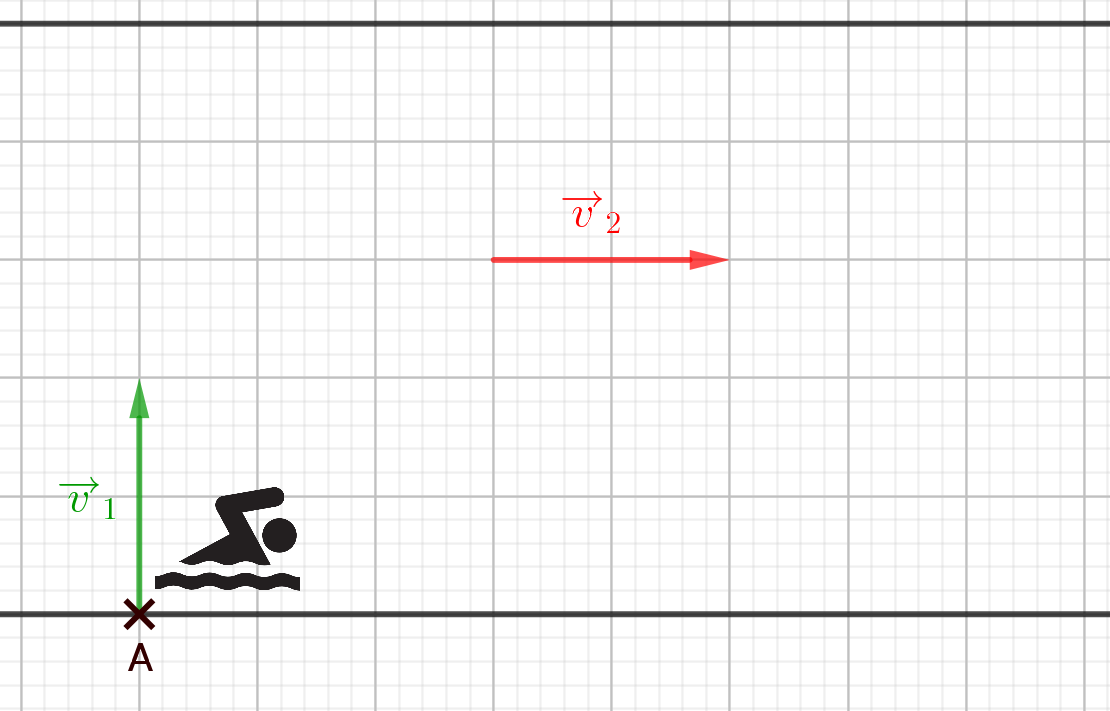
\includegraphics[width=12cm]{evaluation_7_nageur.png}  
\end{center}

Déterminer graphiquement le point sur la berge opposée où arrivera le nageur.




\end{document}
